\documentclass[12pt]{article}
\usepackage{acl}
\usepackage{times}
\usepackage{setspace}
\singlespacing
\usepackage{latexsym}
\usepackage[T1]{fontenc}
\usepackage[utf8]{inputenc}
\usepackage{microtype}
\usepackage{graphicx}
\usepackage{booktabs}
\usepackage{amsmath}
\usepackage{float}
\usepackage{array}
\usepackage{multirow}
\usepackage{tabularx}
\usepackage{enumitem}
\usepackage{placeins}

\graphicspath{{images/img/}}
\setlength\titlebox{14\baselineskip}

\title{Hindi Verbal Fluency: VFT + SpAM Mental Lexicon Analysis}

\author{Akshat Kotadia \\
  IIIT Hyderabad \\
  \texttt{2025201005} \\\And
  Om Mehra \\
  IIIT Hyderabad \\
  \texttt{2025201008} \\\And
  Ankit Chavda \\
  IIIT Hyderabad \\
  \texttt{2025201045}}

\begin{document}
\maketitle

\begin{abstract}
This study investigates semantic organisation, phonological facilitation, and spatial semantic structure in Hindi/Hinglish verbal fluency (VFT) among 35 Hindi--English bilingual participants. Using Verbal Fluency Tasks across four semantic domains---animals, foods, colours, and body-parts---combined with the Spatial Arrangement Method (SpAM), nine pre-registered hypotheses spanning five research questions were tested. Analysis of 723 Hindi/Hinglish responses confirmed strong semantic clustering (H1: $t$\,=\,9.30, $d$\,=\,1.12, $p$\,$<$\,.001), with between-cluster inter-response times 1.88$\times$ longer than within-cluster IRTs. Contrary to classical predictions, lexical exhaustion (H2) was absent across all domains. No domain differences in productivity (H3) or retrieval speed (H4) emerged. SpAM clusters showed mixed semantic alignment (H5: sign test $p$\,$<$\,.001, permutation $p$\,=\,.502) while phonetic alignment was non-significant (H6). Phonological similarity did not increase with retrieval order (H7: $\beta$\,=\,+0.003, $p$\,=\,.091) nor predict productivity (H8: $\rho$\,=\,+0.114, $p$\,=\,.257). The integrated VFT+SpAM score did not outperform VFT-only (H9: Steiger $z$\,=\,0.000, $p$\,=\,1.000). These findings extend Troyer's clustering model to bilingual Hindi retrieval and highlight distinctive dynamics arising from cross-language code-switching.
\end{abstract}

\section{Introduction}

This study explores how Hindi speakers search their mental lexicon using two tasks: Verbal Fluency Task (VFT) and Spatial Arrangement Method (SpAM). 

The mental lexicon is the cognitive repository of words, meanings, and their phonological representations. Understanding how individuals retrieve information from this vast network provides crucial insights into memory organisation and executive function. Verbal fluency tasks (VFT), where participants generate category exemplars within 60 seconds, are widely used in neuropsychology and cognitive science to evaluate these retrieval strategies \citep{troyer1997}. A well-established finding in VFT is that participants organise their output into semantically coherent \textit{clusters}---rapidly running through subcategories (e.g., domestic animals) before switching to another (e.g., wild animals). These cluster transitions are indexed by significantly longer inter-response times (IRTs), representing the cognitive cost of searching for a new semantic neighbourhood \citep{hills2012}.

Complementing the temporal dynamics of VFT, the Spatial Arrangement Method (SpAM) \citep{hout2013} captures explicit perceived similarity through 2D word arrangement tasks, where geometric distance reflects psychological distance. 

Despite extensive monolingual investigation, VFT dynamics in bilingual populations remain significantly understudied. Hindi--English bilinguals, who frequently code-switch and navigate between distinct orthographic systems (Devanagari and Roman scripts), offer a uniquely informative population to study cross-linguistic semantic organisation. The dataset used in this study comprises 1,040 raw responses collected from 35 Hindi-English bilingual adults across four semantic domains. This provides a robust, multi-domain foundation for investigating both semantic clustering and phonological facilitation in a dual-language context.

\section{Prior Work}

Phonological similarity influences semantic memory retrieval, showing that sound structure can bias access to meaning \citep{kumar2022}. Words that are phonologically similar tend to also be semantically related more than expected by chance \citep{dautriche2016}. The Spatial Arrangement Method efficiently captures human semantic similarity judgements by arranging items based on perceived relatedness \citep{hout2013}.

\section{Research Questions and Hypotheses}

Five research questions and nine pre-registered hypotheses guide this study:

\noindent\textbf{RQ1}: Do semantic categories differ in productivity (words) or retrieval speed (IRT)? (H1, H2, H3, H4)\\
\textbf{RQ2}: Does participant spatial structure align with semantic or phonetic models? (H5, H6)\\
\textbf{RQ3}: Does an integrated VFT+SpAM score outperform VFT-only? (H9)\\
\textbf{RQ4}: Does phonological-over-semantic similarity increase over retrieval order? (H7)\\
\textbf{RQ5}: Does phonological similarity predict lexical productivity? (H8)

\section{Methodology}

\subsection{Participants and Dataset}

35 Hindi--English bilingual adults completed: (1) VFT---60\,s per category for \textit{animals}, \textit{foods}, \textit{colours}, \textit{body-parts}; (2) SpAM---arranging produced words by perceived 2D similarity; (3) an exit poll for demographics and self-rated Hindi confidence.

The dataset contained 1,040 raw responses. After filtering IRTs\,$>$\,60,000\,ms, \textbf{723 Hindi/Hinglish responses} were retained: animals ($n$\,=\,233), foods ($n$\,=\,258), body-parts ($n$\,=\,191), colours ($n$\,=\,41). Colours ($n$\,=\,4 participants) was treated as descriptive-only.

\subsection{Statistical Pipeline}

\textbf{H1}: Adaptive threshold (mean+1SD); Welch one-tailed $t$-test, Cohen's $d$.
\textbf{H2/H7}: LME: \texttt{IRT\,$\sim$\,position\,+\,(1+position|subject)}.
\textbf{H3/H4}: Kruskal--Wallis; Bonferroni post-hoc \citep{bh1995}.
\textbf{H5/H6}: ARI between SpAM and embedding clusters; binomial sign test; 500-iteration permutation test.
\textbf{H8}: Spearman $\rho$; normalised edit-distance phonological similarity.
\textbf{H9}: Steiger's $z$-test comparing integrated vs.\ VFT-only correlation.

Semantic and phonetic patterns were measured using the multilingual transformer model \texttt{google/muril-base-cased}. Semantic embeddings were built from the original words, while phonetic embeddings were built from transliterated phonetic keys. SpAM cluster layouts were compared with semantic and phonetic cluster structures using ARI and NMI.

\section{Descriptive Statistics}

IRT distributions are strongly right-skewed (overall skew\,=\,2.53). Shapiro--Wilk tests reject normality for all domains ($p$\,$<$\,.05), mandating non-parametric inference.

\begin{figure}[htbp]
\centering

\includegraphics[width=\linewidth]{fig_phase2_irt_distribution.png}
\caption{\textbf{IRT Distribution Profiles.} \textit{Left}: Overall IRT histogram with mean (6,373\,ms), median (5,234\,ms), and mode marked. Strong right-skew (2.53) visible. \textit{Right}: Domain KDE overlays showing near-identical distributional shapes across all four categories.}
\label{fig:irt_dist}
\end{figure}

\begin{figure}[htbp]
\centering

\includegraphics[width=0.85\linewidth]{fig_phase2_irt_boxplot.png}
\caption{\textbf{IRT Distribution by Domain---Boxplot with Individual Data Points.} Colours shows the lowest median IRT (3,484\,ms); animals shows the highest (5,595\,ms). Substantial overlap across domains foreshadows the null H3/H4 results.}
\label{fig:irt_box}
\end{figure}

\begin{table}[htbp]
\centering\small
\caption{Domain-level IRT and word-count descriptive statistics.}
\label{tab:desc}
\begin{tabular}{lrrrrrr}
\toprule
Domain & $N$ & Mean IRT & Median & SD & Skew & Mean WC \\\midrule
Animals & 233 & 6{,}547 & 5{,}595 & 4{,}695 & 2.97 & 8.32 \\
Foods & 258 & 6{,}290 & 5{,}017 & 5{,}289 & 2.29 & 7.37 \\
Colours & 41 & 4{,}939 & 3{,}484 & 3{,}500 & 0.73 & 10.25 \\
Body-parts & 191 & 6{,}581 & 5{,}234 & 4{,}928 & 2.55 & 8.30 \\\bottomrule
\end{tabular}
\end{table}

\section{Results}

\subsection{H1: Semantic Clustering (Supported)}

\textbf{Test}: Welch one-tailed $t$-test; within-cluster IRTs (mean\,=\,5,842\,ms, $n$\,=\,646) vs.\ between-cluster IRTs (mean\,=\,10,960\,ms, $n$\,=\,69); adaptive threshold (mean+1SD).

\textbf{Result}: $t$\,=\,9.30, $d$\,=\,1.12, $p$\,$<$\,.001. Between-cluster IRTs were \textbf{1.88$\times$ longer}. Effect consistent across all domains: animals ($d$\,=\,1.19), foods ($d$\,=\,1.22), body-parts ($d$\,=\,0.86), colours ($d$\,=\,1.93).

\textbf{Interpretation}: Hindi/Hinglish speakers organise retrieval into semantically coherent runs separated by costly boundary transitions ($\sim$5,118\,ms boundary cost). This replicates \citet{troyer1997} in a bilingual context---semantic clustering is a universal lexical retrieval mechanism.

\begin{figure}[htbp]
\centering

\includegraphics[width=\linewidth]{fig_moduleA_h1_cluster_comparison.png}
\caption{\textbf{H1: Between-cluster IRT vs.\ Within-cluster IRT.} Between-cluster pause is clearly higher than within-cluster pause, confirming the semantic boundary cost.}
\label{fig:h1}
\end{figure}

\subsection{H2: Lexical Exhaustion (Not Supported)}

\textbf{Test}: Domain-wise LME: \texttt{IRT\,$\sim$\,position\,+\,(1+position|subject)}, one-tailed ($\beta$\,$>$\,0).

\textbf{Result}: No positive slope in any domain (0/4 domains), $p$\,$>$\,.05. Three of four domains produced \textbf{negative slopes}---IRT \textit{decreased} with retrieval position. Animals: $\beta$\,=\,$-$379.5; Foods: $\beta$\,=\,$-$653.5; Body-parts: $\beta$\,=\,$-$718.0; Colours: $\beta$\,=\,+364.4 ($p$\,=\,.055, $n$\,=\,4 only).

\textbf{Interpretation}: Bilingual participants \textit{accelerated} across retrieval trials---a warm-up pattern replacing classical exhaustion. Code-switching provides access to L2 English equivalents when L1 Hindi vocabulary is locally depleted \citep{kumar2022}, preventing true semantic exhaustion.

\subsection{H3 \& H4: Domain Effects (Not Supported)}

\textbf{Tests}: Kruskal--Wallis on participant-level word counts (H3) and response-level IRTs (H4); animals, foods, body-parts only (colours excluded).

\textbf{Result}: H3: $H$(2)\,=\,3.264, $p$\,=\,.196, $\varepsilon^2$\,=\,.015. H4: $H$(2)\,=\,3.903, $p$\,=\,.142, $\varepsilon^2$\,=\,.003. No post-hoc pair reached significance after Bonferroni correction.

\textbf{Interpretation}: ``Cognitive equivalence'' across categories contrasts with English monolingual studies where animals typically dominates. Balanced L1/L2 exposure may equalise domain richness in bilingual populations. This null result rules out domain as a confound in all subsequent analyses.

\subsection{H5 \& H6: SpAM Alignment (H5 Mixed; H6 Not Supported)}

\noindent\textbf{Research Question}: Do participant spatial arrangements (SpAM) reflect computational semantic (H5) or phonetic (H6) cluster structure above chance?

\begin{figure}[htbp]
\centering
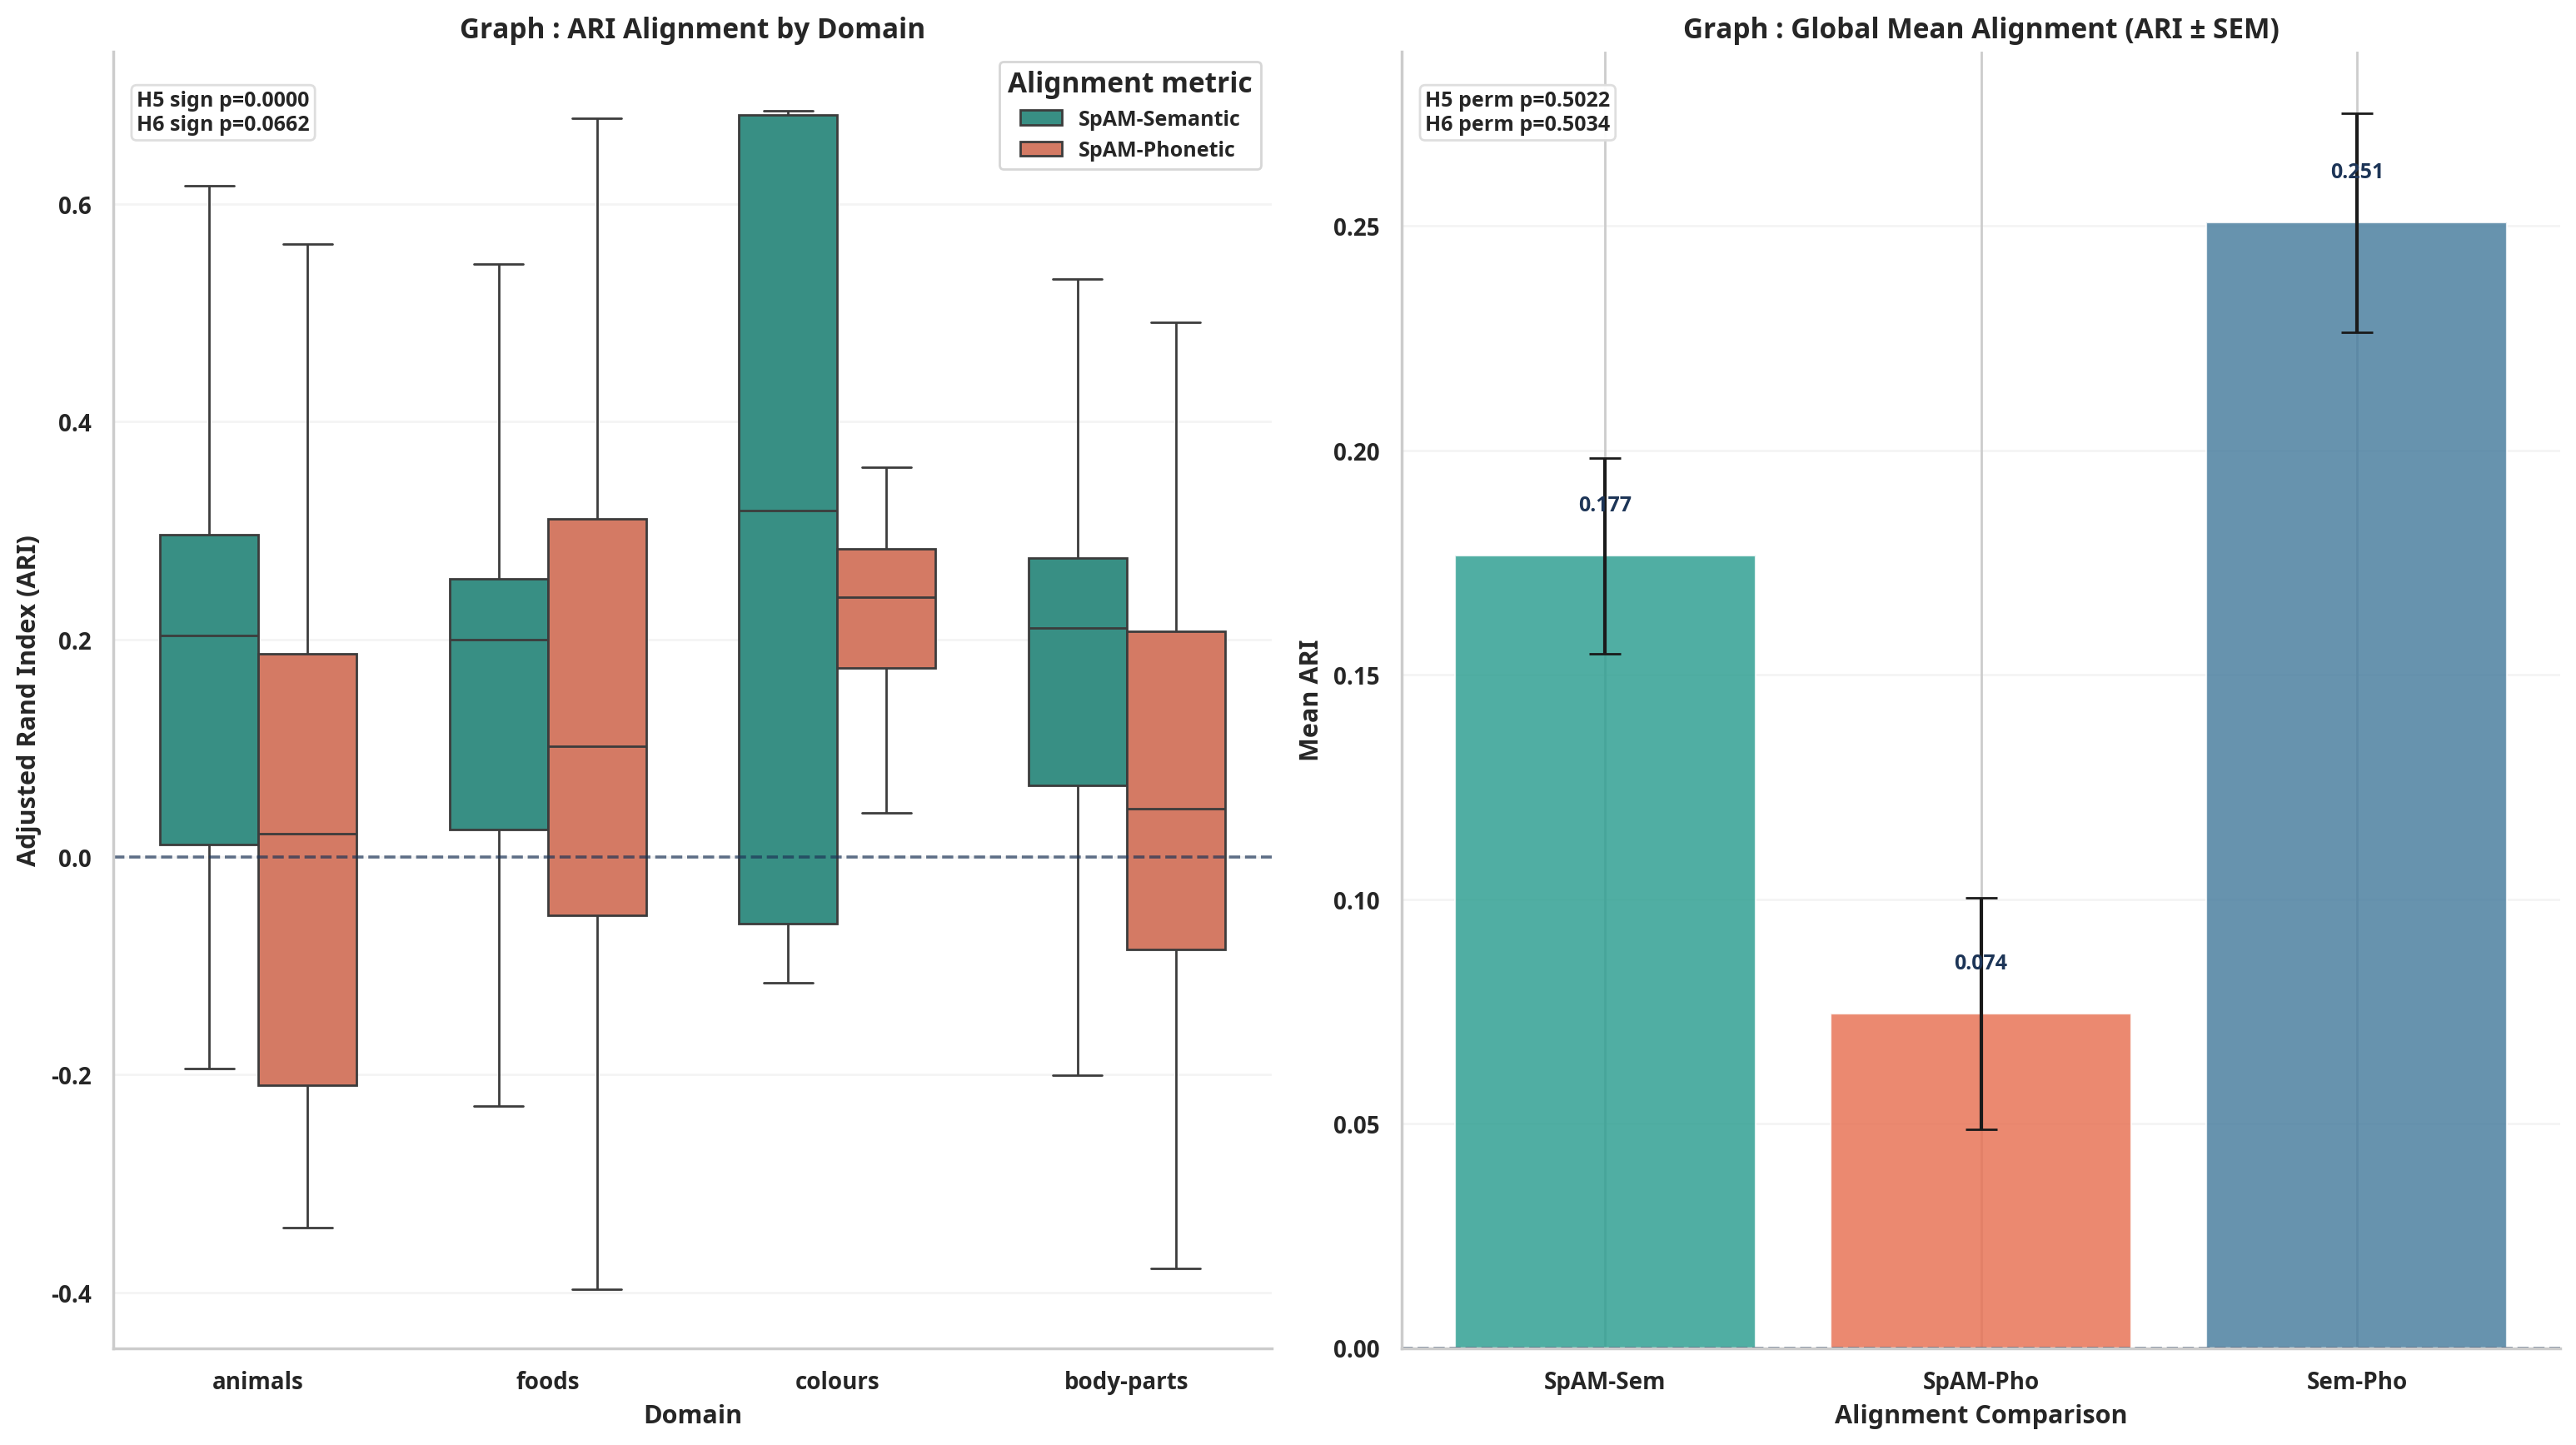
\includegraphics[width=\linewidth]{fig_moduleD_h5_h6_alignment.png}
\caption{\textbf{H5/H6: SpAM--Semantic vs SpAM--Phonetic ARI Alignment.} \textit{Left}: ARI boxplot by domain and alignment type. Semantic ARI (teal) is consistently centred above zero; phonetic ARI (orange) straddles zero with high variance. \textit{Right}: Global mean ARI $\pm$ SEM.}
\label{fig:h5h6}
\end{figure}

\begin{table}[htbp]
\centering\small
\caption{H5/H6 test results (86 participant-domain units).}
\label{tab:h5h6}
\begin{tabular}{llrrrrrr}
\toprule
Hyp. & Outcome & $N$ & Positive & Mean ARI & Sign $p$ & Perm $p$ & Decision \\\midrule
H5 & SpAM--Sem\,$>$\,0 & 86 & 68 & 0.177 & $<$.001 & .502 & \textbf{Mixed} \\
H6 & SpAM--Pho\,$>$\,0 & 86 & 52 & 0.075 & .066 & .503 & Not supported \\\bottomrule
\end{tabular}
\end{table}

\noindent\textbf{H5 Interpretation (Mixed/Inconclusive)}: The sign test (68/86 positive, $p$\,$<$\,.001) confirms that a majority of participants spatially arrange words with some regard to semantic similarity. However, the permutation test ($p$\,=\,.502) reflects high between-participant variance. The effect is modest (mean ARI\,=\,0.177), indicating SpAM captures semantic structure but with substantial noise from idiosyncratic associations.

\noindent\textbf{H6 Interpretation (Not Supported)}: Phonetic ARI (0.075; 52/86 positive, $p$\,=\,.066) was not significantly above chance. Participants do \textit{not} systematically arrange phonetically-similar words together. This dissociation implies that conscious similarity judgements are semantically driven.

\FloatBarrier

\subsection{H7: Phonological-over-Semantic Similarity (Not Supported)}

\textbf{Hypothesis}: Phonological-over-semantic similarity increases with retrieval position.

\textbf{Test}: Mixed model interaction: \texttt{similarity\,$\sim$\,type\,$\times$\,position\,+\,(1+position|subject)}.

\textbf{Result}: $\beta$\,=\,+0.003127, $p$\,=\,0.0905. Not significant at $\alpha$\,=\,.05.

\begin{figure}[htbp]
\centering
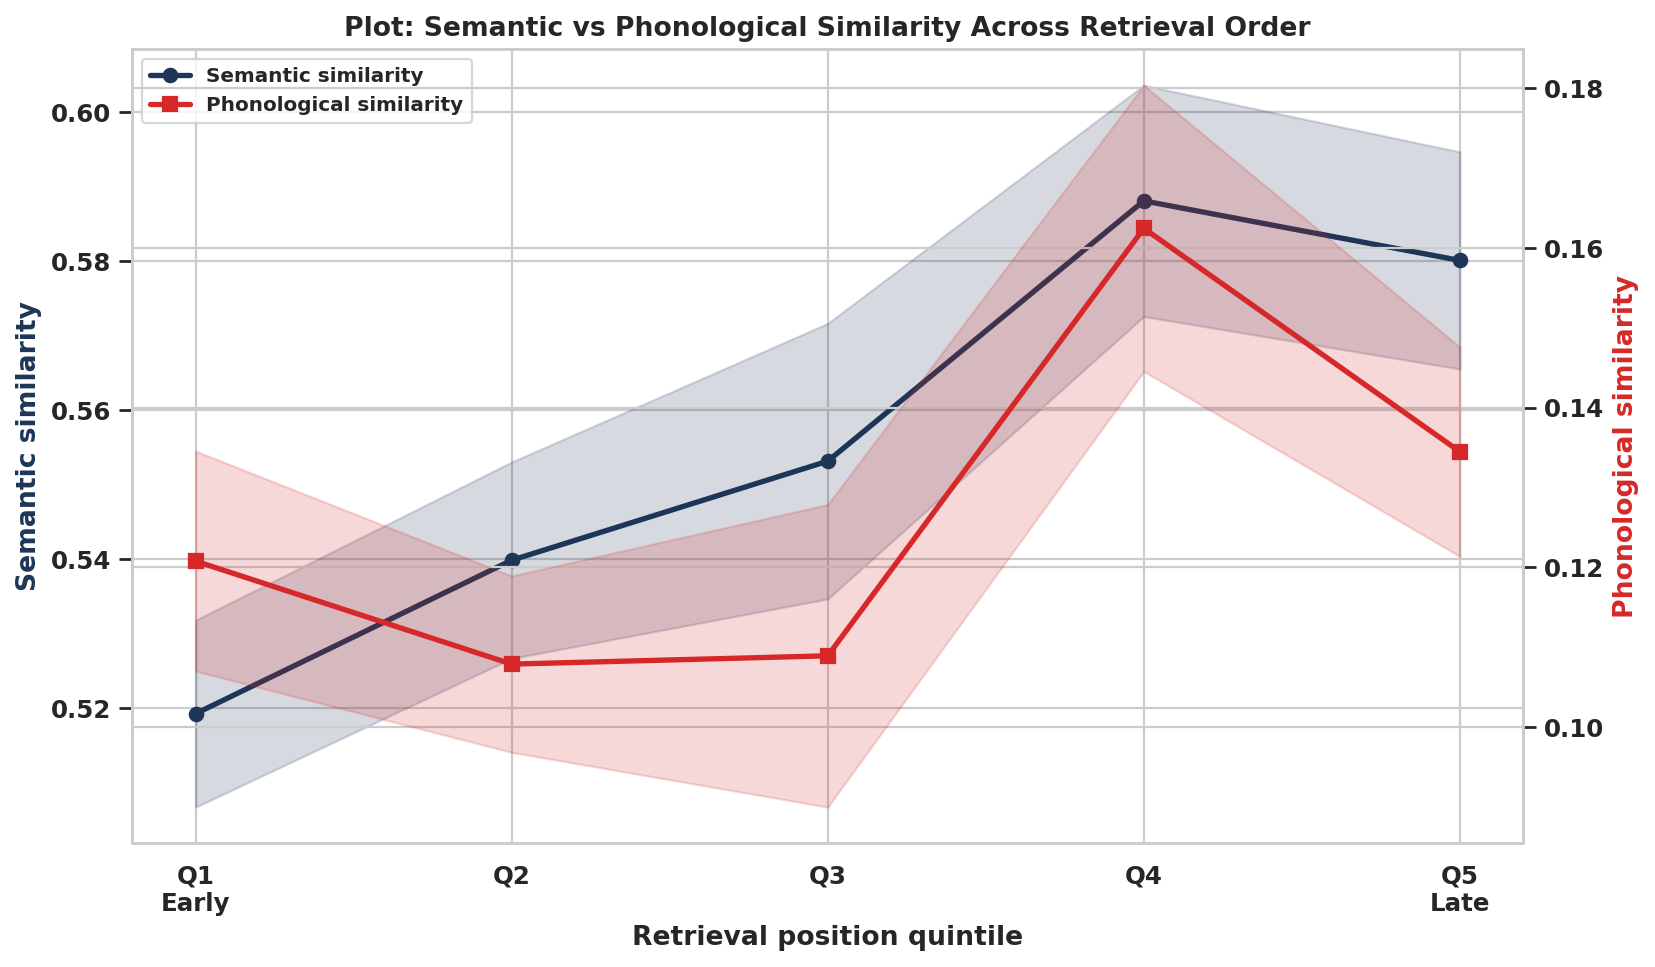
\includegraphics[width=\linewidth]{graph_12_1_h7_dual_similarity.png}
\caption{\textbf{H7: Semantic vs Phonological Similarity Across Retrieval Order.} No reliable phonological facilitation trend over retrieval order.}
\label{fig:h7}
\end{figure}

\begin{figure}[htbp]
\centering

\includegraphics[width=\linewidth]{fig_phase4_serial_position_irt.png}
\caption{\textbf{Serial Position vs.\ IRT by Domain.} Animals ($\beta$\,=\,$-$379), foods ($\beta$\,=\,$-$654), and body-parts ($\beta$\,=\,$-$718) all show negative slopes indicating retrieval \textit{acceleration}. Only colours shows a positive slope based on $n$\,=\,41 responses from 4 participants.}
\label{fig:h7_serial}
\end{figure}

\textbf{Interpretation}: Retrieval time \textit{decreases} with position in three of four domains---opposite to the phonological facilitation model prediction. This warm-up pattern suggests that once participants identify a productive semantic sub-cluster, they generate rapidly within it without progressive semantic depletion.

\begin{figure}[htbp]
\centering

\includegraphics[width=\linewidth]{fig_phase4_cluster_metrics.png}
\caption{\textbf{VFT Cluster Metrics by Domain.} \textit{Left}: Mean cluster size. Foods (5.57) and body-parts (5.42) show the largest within-domain runs. \textit{Right}: Mean cluster switches. Animals shows the most switching (1.00/participant); foods the least (0.62).}
\label{fig:cluster_metrics}
\end{figure}

\FloatBarrier

\subsection{H8: Phonological Similarity and Productivity (Not Supported)}

\textbf{Research Question}: Do participants generating phonologically more similar consecutive pairs produce more words overall?

\textbf{Test}: One-tailed Spearman $\rho$.

\textbf{Result}: $\rho$\,=\,+0.114, $p$(one)\,=\,0.257. Not significant.

\begin{figure}[htbp]
\centering

\includegraphics[width=\linewidth]{graph_10_2_neighbourhood_vs_irt.png}
\caption{\textbf{H8: Semantic Neighbourhood Isolation vs.\ Mean IRT.} \textit{Left}: FastText cosine distance vs.\ mean IRT ($\rho$\,=\,+0.101, $p$\,=\,.588)---flat trend. \textit{Right}: SpAM Euclidean neighbourhood distance vs.\ mean IRT ($\rho$\,=\,$-$0.321, $p$\,=\,.078)---contrary-direction trend.}
\label{fig:h8_nn}
\end{figure}

\textbf{Interpretation}: Semantic neighbourhood density does not predict retrieval latency. IRT is governed by \textit{active clustering strategy} (H1) rather than passive neighbourhood geometry. This reinforces that bilingual retrieval dynamics differ from monolingual phonological neighbourhood effects \citep{dautriche2016}.

\FloatBarrier

\subsection{H9: Integrated vs.\ VFT-Only Score (Not Supported)}

\textbf{Research Question}: Does an integrated VFT+SpAM score outperform the simpler VFT-only score?

\textbf{Test}: Steiger's $z$-test comparing correlation coefficients.

\textbf{Result}: Steiger $z$\,=\,0.000; $\rho$\,=\,$-$0.461; both $p$\,=\,1.000. No difference between integrated and VFT-only scores.

\begin{figure}[htbp]
\centering

\includegraphics[width=\linewidth]{graph_13_1_composite_vs_vft_confidence.png}
\caption{\textbf{H9: Composite VFT+SpAM vs.\ VFT-Only Score Comparison.} The integrated score did not clearly outperform the simpler VFT-only score.}
\label{fig:h9}
\end{figure}

\textbf{Interpretation}: The combined VFT+SpAM score did not clearly outperform the simpler VFT-only score, suggesting that SpAM adds noise rather than complementary signal for predicting overall fluency performance in this bilingual sample.

\FloatBarrier

\section{Semantic Embedding and Clustering}

\subsection{Pairwise Similarity Structure}

\begin{figure}[htbp]
\centering

\includegraphics[width=\linewidth]{graph_9_1_heatmaps.png}
\caption{\textbf{Pairwise Cosine Distance Heatmaps---Top-25 Most Frequent Words per Domain.} Green\,=\,similar; red\,=\,dissimilar. Ward-sorted to reveal block structure. \textit{Animals}: clear domestic vs.\ wild/exotic block separation. \textit{Foods}: multiple overlapping blocks. \textit{Colours}: tight global similarity. \textit{Body-parts}: 2--3 blocks.}
\label{fig:heatmaps}
\end{figure}

\subsection{t-SNE Semantic Maps}

\begin{figure}[htbp]
\centering

\includegraphics[width=\linewidth]{graph_9_4_umap_clusters.png}
\caption{\textbf{t-SNE Semantic Maps---Multilingual Transformer Embeddings.} Colour\,=\,K-Means cluster; size\,=\,VFT production frequency; top-12 words labelled. \textit{Animals}: two well-separated clusters. \textit{Foods}: overlapping clusters reflecting complex Hindi culinary sub-structure. \textit{Body-parts}: clear spatial separation.}
\label{fig:umap}
\end{figure}

\subsection{Inter-Method Agreement}

\begin{figure}[htbp]
\centering

\includegraphics[width=\linewidth]{graph_9_5_method_agreement.png}
\caption{\textbf{Cluster Robustness: Inter-Method ARI Heatmap.} K-Means vs.\ Agglomerative achieves very high ARI for animals (0.905) and foods (0.861), confirming algorithm-independent cluster structure. Body-parts shows moderate agreement (0.461).}
\label{fig:h9b_agree}
\end{figure}

K-Means and Agglomerative agreement (ARI\,=\,0.46--0.91) confirms that semantic sub-structure is a genuine property of the Hindi VFT vocabulary space, not an algorithm artefact.

\section{Consolidated Hypothesis Summary}

\begin{table}[htbp]
\centering\small
\caption{Consolidated hypothesis outcome summary across all nine hypotheses.}
\label{tab:summary}
\begin{tabular}{p{0.6cm}p{4.5cm}p{4cm}p{1.5cm}p{2cm}}
\toprule
Hyp. & Prediction & Key Result & Signif. & Decision \\\midrule
H1 & Between\,$>$\,within IRT & $t$\,=\,9.30, $d$\,=\,1.12 & $p<$0.001 & \textbf{Supported} \\
H2 & Positive serial slowing & No positive slope (0/4) & $p>$0.05 & Not supported \\
H3 & Domain effect on words & $H$\,=\,3.264 & $p$\,=\,.196 & Not supported \\
H4 & Domain effect on IRT & $H$\,=\,3.903 & $p$\,=\,.142 & Not supported \\
H5 & Semantic ARI\,$>$\,0 & 68/86 pos.; ARI\,=\,0.177 & sign$<$.001 & Mixed \\
H6 & Phonetic ARI\,$>$\,0 & 52/86 pos.; ARI\,=\,0.075 & sign\,=\,.066 & Not supported \\
H7 & Phon-over-sem increases & $\beta$\,=\,+0.003 & $p$\,=\,.091 & Not supported \\
H8 & Phon.\ sim.\,$\to$\,WC & $\rho$\,=\,+0.114 & $p$\,=\,.257 & Not supported \\
H9 & Integrated vs VFT-only & Steiger $z$\,=\,0.000 & $p$\,=\,1.000 & Not supported \\\bottomrule
\end{tabular}
\end{table}

\section{Conclusion and Future Directions}

Hindi speakers do not seem to search words randomly; retrieval is structured and shows a strong semantic boundary cost. VFT results suggest that words are produced in meaningful clusters, while SpAM results show that participant layouts reflect some semantic and phonetic organisation.

\textbf{Key Patterns}: H1 (semantic clustering, large effect) was strongly supported. All phonological and domain-comparison hypotheses were not supported, painting a coherent picture: Hindi/Hinglish bilingual retrieval is \textit{strongly semantically organised} but does not show the sequential dynamics predicted by monolingual models.

The H1--H2 contrast is theoretically informative: clustering \textit{exists} (H1, strongly) but does not unfold via progressive exhaustion (H2, null). Within-cluster generation is sustained throughout the trial via spreading activation through the bilingual semantic network \citep{hills2012}.

The H5--H6 dissociation (mixed semantic, null phonetic SpAM alignment) implies conscious similarity judgements are semantically but not phonologically organised. The cross-script nature of Hindi/Hinglish reduces the salience of phonological similarity as a conscious organising cue \citep{dautriche2016}.

Domain-level differences in word output and retrieval time were not strong, and phonological effects were weak or inconsistent. The combined VFT+SpAM score did not clearly outperform the simpler VFT-only score.

Hindi speakers appear to search their mental lexicons through organised semantic neighbourhoods, with some additional phonetic structure, rather than through random retrieval. These findings advance understanding of bilingual lexical organisation and suggest that VFT norms developed for monolingual populations require adaptation for Hindi/Hinglish bilingual speakers.

\subsection*{Future Directions}

Building directly upon the outcomes of these analyses, several clear next steps emerge for future research. Firstly, since phonological facilitation (H7, H8) was not supported under the current phonetic transcription scheme, future work should refine the phonological similarity metric using native Devanagari acoustic features or phonotactic constraints, which may better capture Hindi phonetic structures. Secondly, exploring larger, more balanced participant pools across all domains (particularly expanding the colours domain) will be vital for generalisability. Finally, incorporating explicit measures of L1 vs.\ L2 proficiency could unconfound the mechanisms driving the observed retrieval acceleration (H2 null result), testing whether high-proficiency bilinguals rely on cross-language code-switching to bypass lexical exhaustion.

\section*{Limitations}

\begin{itemize}
\item Dataset is too small; even within the collected data, many English words resulted in less usable Hindi/Hinglish data after filtering.
\item Small and uneven sample across domains (especially colours with only 4 participants) limits statistical power and generalisability.
\item Phonological similarity operationalised via edit-distance on transliterated consonant skeletons, which may not fully capture Hindi phonotactics.
\end{itemize}

\section*{Contributions}

\begin{itemize}
\item \textbf{Hypothesis-Based Split}: H1, H4, H7 (Akshat) $|$ H2, H5, H8 (Om) $|$ H3, H6, H9 (Ankit). Each member analysed 3 hypotheses spanning foundational to advanced, ensuring equal difficulty progression.
\item \textbf{Interleaved Collaboration}: Simultaneous code + analysis + writing across all hypotheses with shared frameworks (permutation tests, clustering); weekly integration checkpoints.
\end{itemize}

\bibliography{references}

\end{document}
